\section{Dokumentation}

% Was mussten die Teilnehmer machen?
Im ersten Teil der Umfrage mussten die Teilnehmenden zu zwei Aussagen verschiedene Kriterien bewerten.
Diese Kriterien wurden gewählt basierend auf Erfahrung als Entwickler als auch Beobachtungen vieler
Dokumentationen während der manuellen Datenerfassung zu aus Kapitel
\ref{ssec:manuelle_datenerfassung_dokumentation}.


\bigskip
\noindent
Die erste Aussage war \textit{"Wie wichtig sind Ihnen folgende Aspekte der OSS-Dokumentation"}, mit den Punkten:
\begin{multicols}{2}
    \begin{itemize}
        \setlength\itemsep{0em}
        \item Übersichtlichkeit
        \item Einfache Sprache
        \item Live-Demos
        \item Übersetzungen (z.B. Englisch -> Deutsch)
        \item Das Vorhandsein einer Getting Started Page
        \item Code Beispiele
        \item Strukturierung der Dokumentation
        \item []
    \end{itemize}
\end{multicols}

\bigskip
\noindent
Die zweite Aussage war \textit{"Die folgenden Punkte würden mich von der Nutzung eines OSS-Projekts
    abhalten oder mich möglicherweise dazu veranlassen, nach Alternativen zu suchen."}, mit den Punkten:

\begin{multicols}{2}
    \begin{itemize}
        \setlength\itemsep{0em}
        \item Keine Code Beispiele
        \item Schlecht strukturierte Dokumentation
        \item Dokumentation zu komplex
        \item Fehlende Übersetzung (z.B. fehlende deutsche Übersetzung)
        \item Fehlende Getting Started Page
    \end{itemize}
\end{multicols}



\bigskip
\noindent
% More Detail
Die Aussagen wurden auf einer 5-Punkte Skala bewertet, hierbei entspricht 1 \textit{Stimme gar nicht zu}
und 5 \textit{Stimme vollkommen zu}. Um die Aussagen miteinander zu vergleichen, wurde jeweils der
Mittelwert berechnet.

% Conclusion
Die zwei wichtigsten Aspekte einer Guten Dokumentation sind laut den Befragten, Code Beispiele und
Übersichtlichkeit in beiden Fällen mit einem durchschnittlichen Wert von 4,36. Gefolgt von guter 
Struktur (4,09) und
das Vorhandensein eines \textit{Getting Started} (3,98). Einfache Sprache (3,08) und Live-Demos spielt für
die Befragten eine weniger wichtige Rolle. 
Übersetzungen belegen mit 1,53 den letzten Platz und spielt somit die unwichtigste Rolle in einer 
guten Dokumentation. 


Die zweite Aussage war \textit{"Die folgenden Punkte würden mich von der Nutzung eines OSS-Projekts
    abhalten oder mich möglicherweise dazu veranlassen, nach Alternativen zu suchen."} Am höchsten bewertet
wurde der Punkt \textit{Fehlende Code Beispiele} (4,07) und ist somit der wichtigste Teil einer guten
Dokumentation, gefolgt von schlechter Struktur (3,91). 
Eine komplexe Dokumentation oder das Fehlen einer Getting Started Seite wurde hierbei als mittelmäßig kritisch 
eingestuft, mit einer durchschnittlichen Bewertung von 3,29 bzw. 3,10. Das Fehlen einer Übersetzung ist mit 1,37
das unwichtigste Kriterium.
In den Abbildungen \ref{abb:GuteDoku_BarChart} und
\ref{abb:SchlechteDoku_BarChart} wird das Meinungsbild der Teilnehmer grafisch dargestellt.

% Interpretation beider Fragen.
Zusammenfassend kann man sagen, dass Code Beispiele ein Must Have einer Dokumentation ist.
Das Vorhandensein wird als wichtig eingestuft, während das Fehlen dazu führen könnte, dass Nutzer
zu alternativen greifen würden. Übersetzungen hingegen werden als gleichgültig betrachtet, das
Vorhandensein bietet wenig Mehrwert, die Abwesenheit wird nicht als kritisch betrachtet.

% ---------------------------------------------------- %
% Likert to Kano (kinda)
% https://www.eric-klopp.de/texte/die-kano-methode.php
% ---------------------------------------------------- %


% ----------------------------------------- FreitextFeld ----------------------------------------- %
\bigskip
\noindent
Beide Fragen hatten jeweils ein Freitextfeld, indem die Teilnehmenden die Möglichkeit hatten weitere
Aspekte einer guten bzw. schlechten Dokumentation zu nennen. Diese Freitextfelder waren optional und
wurden von 95 bzw. 71 der gesamten 308 Teilnehmenden genutzt.
Alle Einträge wurden kategorisiert und zusammengefasst.

% Most Used Words
In der Tabelle \ref{tab:freitext_felder_ergebnisse} finden sich die am häufigsten genannten
Punkte. Aktualität, Vollständigkeit und UX waren die am meisten genannten Eigenschaften
bezüglich guter Dokumentation, die jeweiligen Pendants, veraltete Dokumentation, unvollständige
Dokumentation und schlechte UX waren die häufigsten genannten Gründe, um ein OSS Projekt nicht zu
nutzten. Diese drei Merkmale vervollständigen somit die vorhin erwähnten \textit{Must-Haves} einer
guten Dokumentation.

\bigskip
\begin{table}[h]
    \begin{tabular}{lcllc}
        \cline{1-2} \cline{4-5}
        \textbf{Gute Dokumentation} & \multicolumn{1}{l}{\textbf{Erwähnungen}} & \hspace{1cm} & \textbf{Schlechte Dokumentation}   & \multicolumn{1}{l}{\textbf{Erwähnungen}} \\ \cline{1-2} \cline{4-5}
        Aktualität                  & 28                                       &              & Veraltet                           & 25                                       \\
        Vollständigkeit             & 21                                       &              & Unvollständig                      & 15                                       \\
        Gute UX                     & 14                                       &              & Schlechte UX                       & 11                                       \\
        Versionierung               & 10                                       &              & Fehlerhaft                         & 7                                        \\
        Changelog vorhanden         & 6                                        &              & Keine Doku vorhanden               & 6                                        \\
        Gute Code Beispiele         & 5                                        &              & Code Beispiele funktionieren nicht & 5
    \end{tabular}%
    \caption{Häufigste Erwähnungen der Freitexter}
    \label{tab:freitext_felder_ergebnisse}
\end{table}


\subsubsection*{Anmerkung:}
\textit{Im Fall von UX wurden folgende Punkte zusammengefasst: Suchfunktion/Verlinkung, Design und
Übersichtlichkeit.}


\bigskip
\bigskip
\noindent
Die abschließende Frage zum Thema Dokumentation war: \textit{"Hat eine schlechte Dokumentation Sie jemals
    dazu gebracht, ein alternatives Projekt zu wählen?"}. 81\% der Teilnehmen haben diese Frage mit
\textit{"Ja"} beantwortet. 


% Gutes Zitat tbh.
% "Gar keine Dokumentation ist ein Zeichen von fehlendem Engagement/Einsatz - nicht vertrauenswürdig"


% ------------------------------------------ Bar Charts ------------------------------------------ %
\begin{figure}[h]
    \centering
    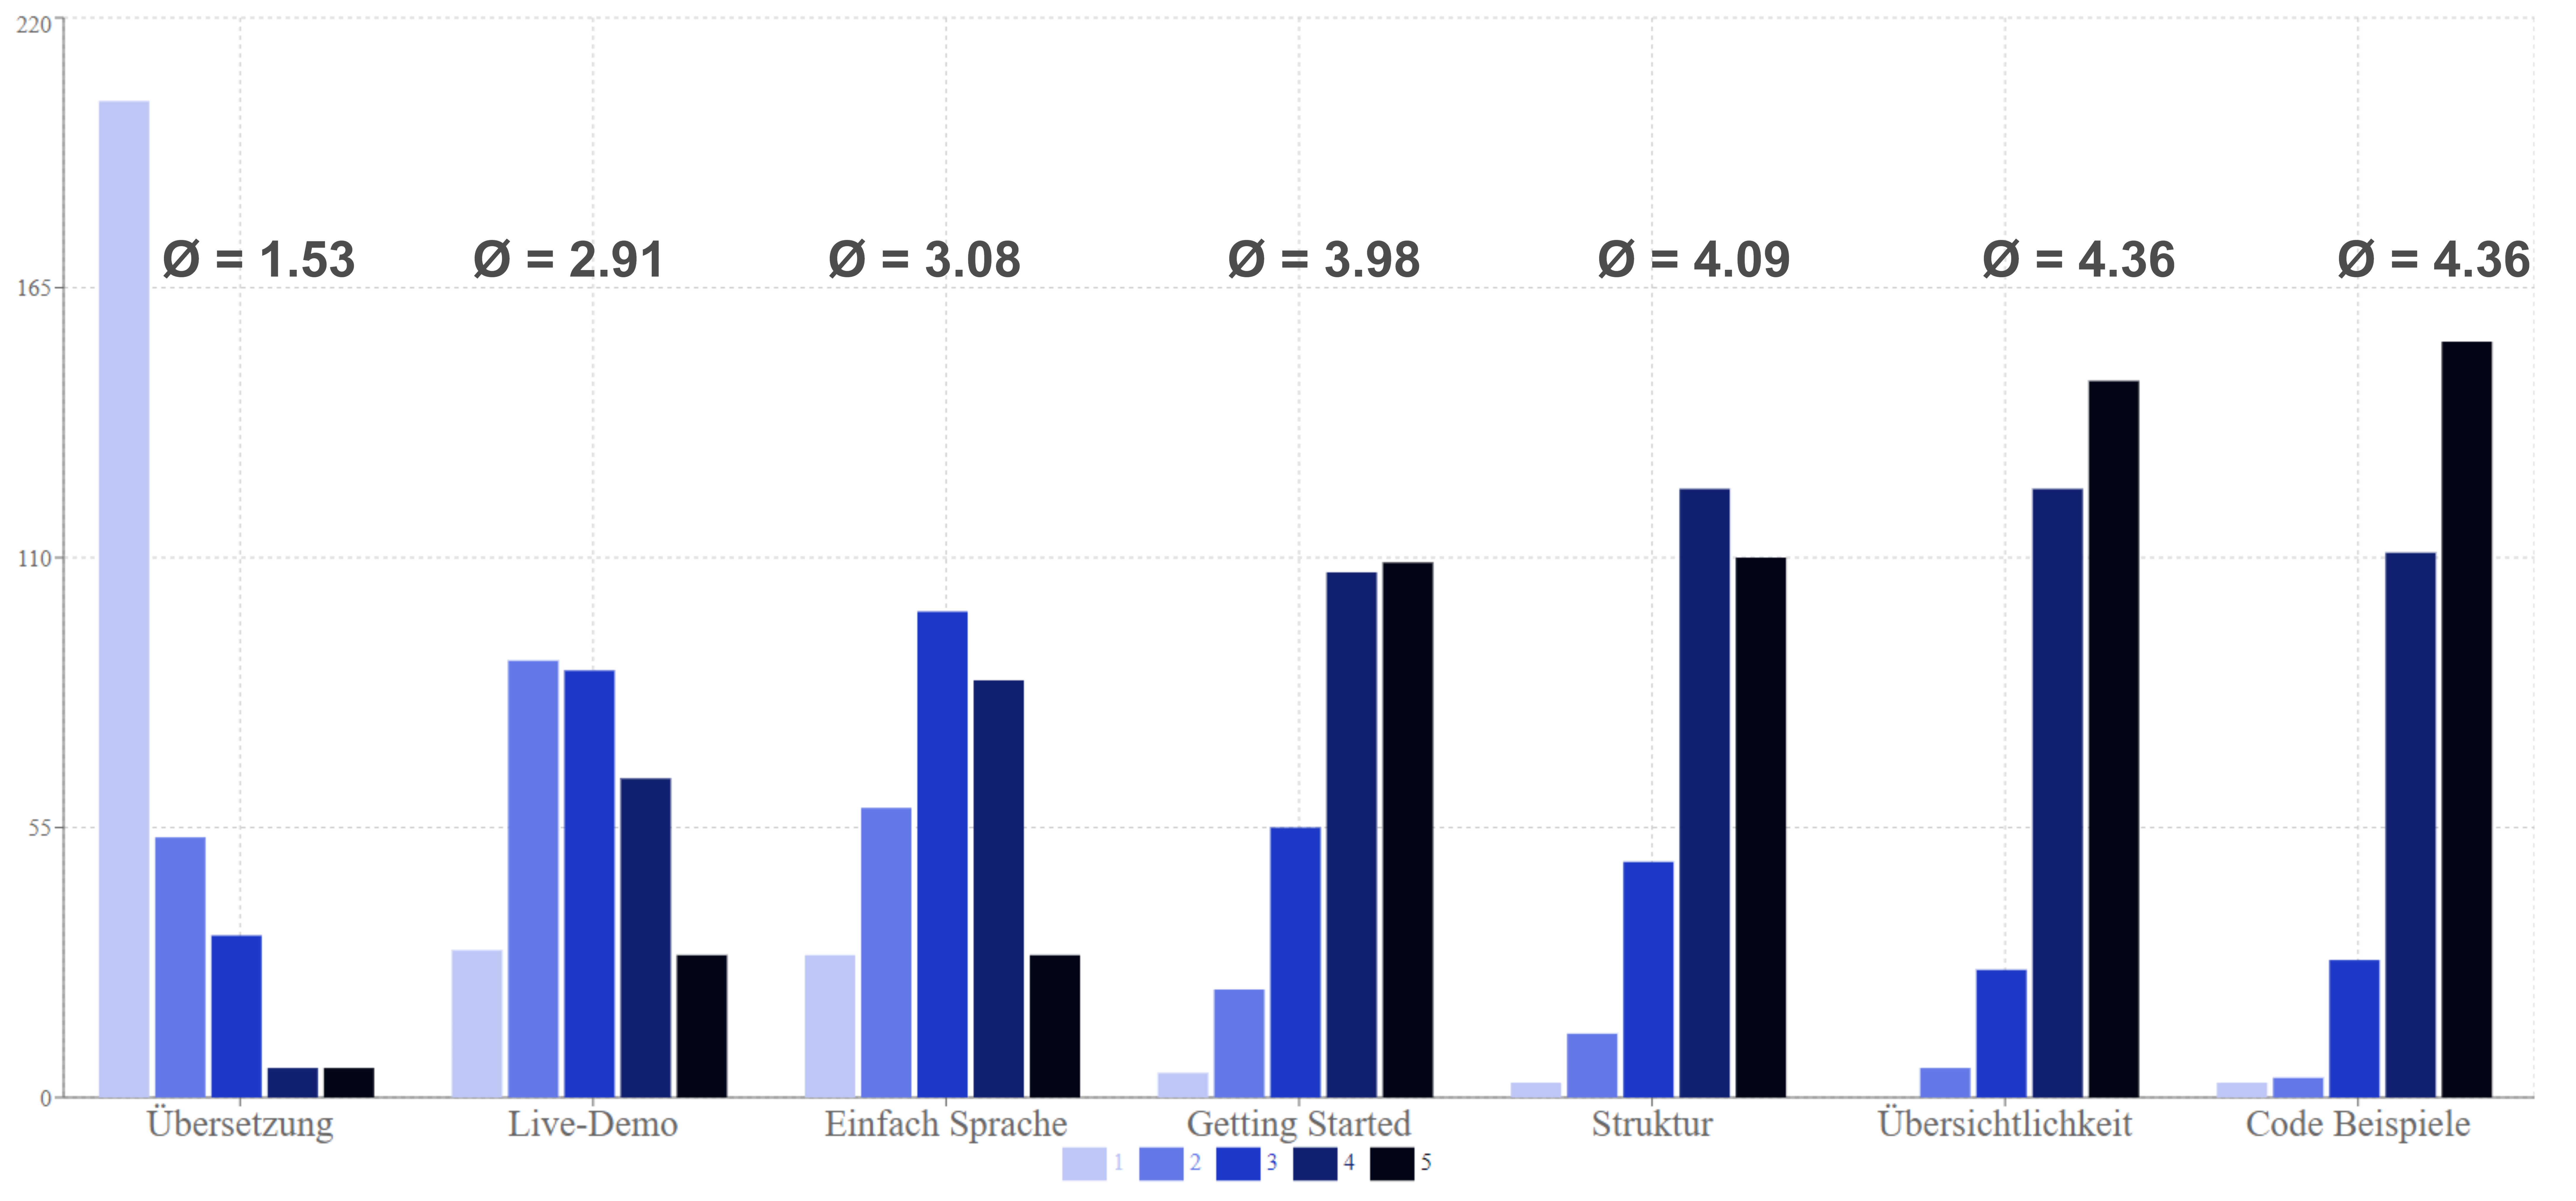
\includegraphics[scale=0.05]{figures/05/GuteDoku_BarChart.png}
    \caption{Antworten: Was zeichnet Gute Dokumentation aus?}
    \label{abb:GuteDoku_BarChart}
\end{figure}

\begin{figure}[h]
    \centering
    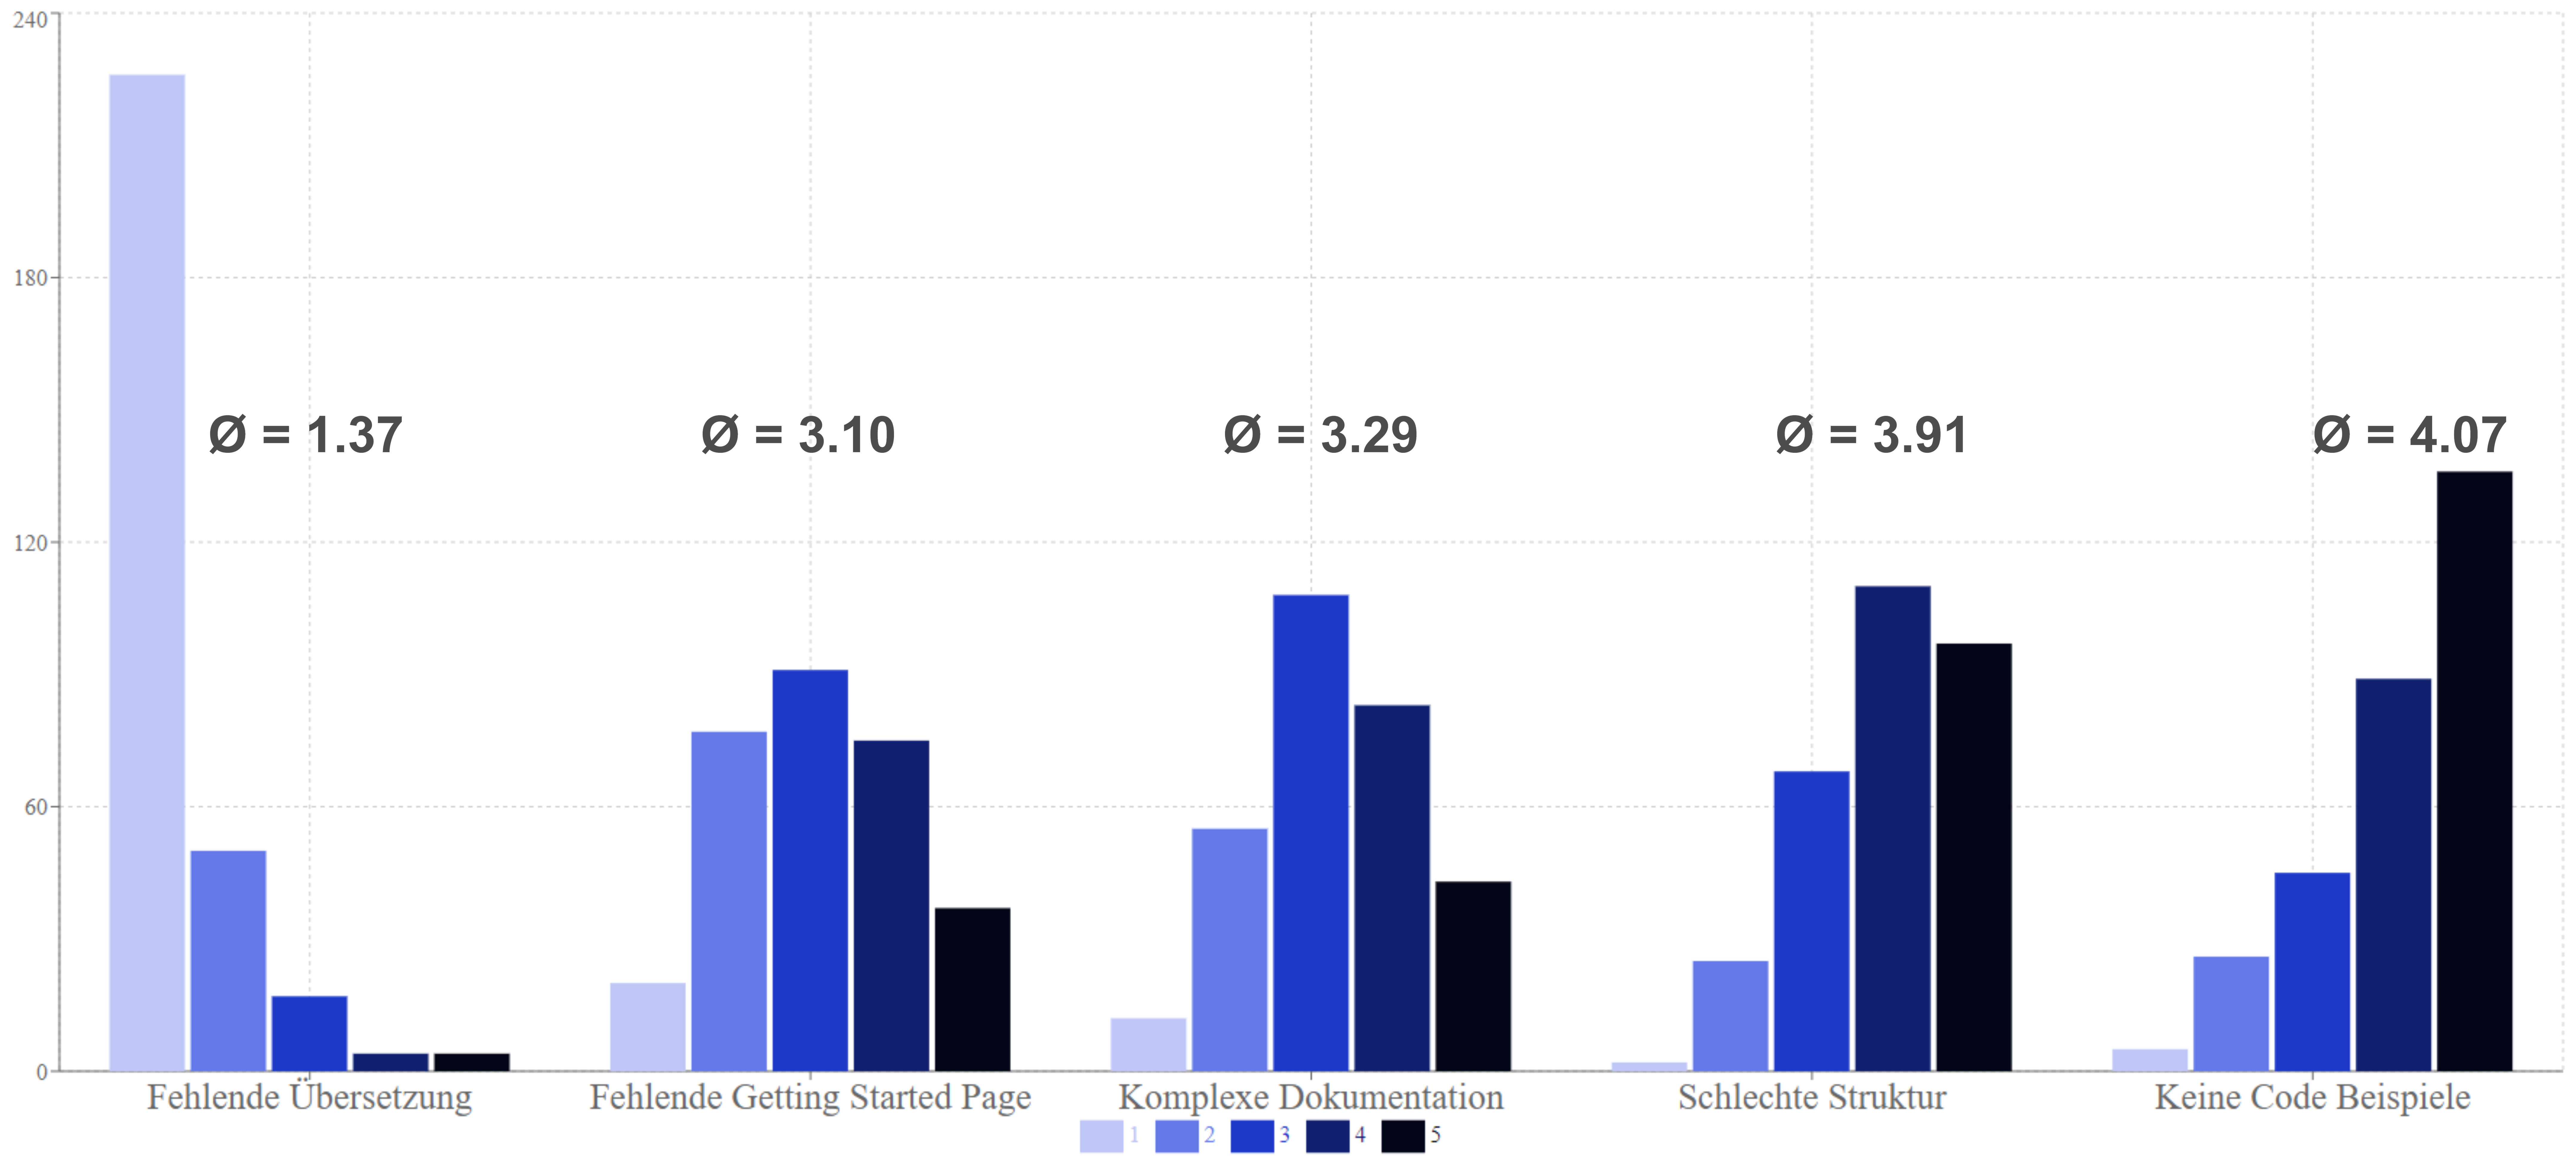
\includegraphics[scale=0.05]{figures/05/SchlechteDoku_BarChart.png}
    \caption{Antworten: Was zeichnet Gute Dokumentation aus?}
    \label{abb:SchlechteDoku_BarChart}
\end{figure}